\documentclass[dvipsnames]{article}
\usepackage[english]{babel}
\usepackage{multirow}
\usepackage[letterpaper,top=2cm,bottom=2cm,left=3cm,right=3cm,marginparwidth=1.75cm]{geometry}
\usepackage{amsmath}
\usepackage{graphicx}
\usepackage{minted}
\usepackage{amsthm}
\usepackage{mathtools}
\usepackage[colorlinks=true, allcolors=blue]{hyperref}
\usepackage{fancyhdr}
\usepackage{enumerate}

\usepackage{tikz}
\usetikzlibrary{shapes}
\usetikzlibrary{arrows}

\tikzset{
  treenode/.style = {align=center, inner sep=0pt, text centered,
    font=\sffamily},
  avl_node/.style = {treenode, circle, black, draw=black,
    text width=1.5em, very thick},% arbre rouge noir, noeud rouge
  black_node/.style = {treenode, circle, white, font=\sffamily\bfseries, draw=black,
    fill=black, text width=1.5em},% arbre rouge noir, noeud noir
  red_node/.style = {treenode, circle, red, draw=red,
    text width=1.5em, very thick},% arbre rouge noir, noeud rouge
  nil_leaf/.style = {treenode, rectangle, draw=black, fill=black,
    minimum width=0.3em, minimum height=0.3em}% arbre rouge noir, nil
}

\begin{document}
\section*{Week 7. Problem set (solutions by \textcolor{blue}{Karim Khabibrakhmanov})}

\thispagestyle{fancy}
\lhead{Karim Khabibrakhmanov (\texttt{k.khabibrakhmanov@innopolis.university}), group B24-DSAI-05}

\begin{enumerate}
  \item Insert the following keys into an initially empty AVL tree \cite[\S 11.3]{Goodrich2014}:
    \[
      2, 3, 29, 5, 11, 23, 13, 17, 19, 7
    \]
    For each insertion:
    \begin{itemize}
      \item show the \emph{state of the tree} \textbf{after} the insertion
      \item specify the \emph{number of rotations} performed during the insertion
      % \item specify the \emph{number of recolorings} performed during the insertion
      % (\textbf{do not} count recoloring of the root node, only count those included in case 1~\cite[Figure~13.5]{Cormen2022})
    \end{itemize}

    Depict each tree using the array representation for binary trees.
    For example, consider the following AVL tree:

    \begin{center}
      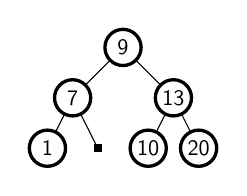
\begin{tikzpicture}[scale=.8, transform shape, level distance = 0.8cm]
        % [->,>=stealth',level/.style={sibling distance = 2cm/#1, level distance = 0.8cm}]
        \tikzstyle{level 1}=[sibling distance=16mm]
        \tikzstyle{level 2}=[sibling distance=8mm]
      \node [avl_node] {9}
          child{ node [avl_node] {7}
            child{ node [avl_node] {1}
            }
            child{ node [nil_leaf] {} }
          }
          child{ node [avl_node] {13}
            child{ node [avl_node] {10} }
            child{ node [avl_node] {20} }
          }
      ;
      \end{tikzpicture}
    \end{center}

    The tree above must be depicted as the following array:

    \begin{center}
    \begin{tabular}{|c|c|c|c|c|c|c|c|c|c|c|c|c|c|c|}
      \hline
        \makebox[\widthof{0}][c]{9}
      & \makebox[\widthof{0}][c]{7}
      & \makebox[\widthof{0}][c]{13}
      & \makebox[\widthof{0}][c]{1}
      & \makebox[\widthof{0}][c]{--}
      & \makebox[\widthof{0}][c]{10}
      & \makebox[\widthof{0}][c]{20}
      \\
      \hline
    \end{tabular}
    \end{center}

    \color{blue}
    \textbf{Answer:} \\
    \begin{center}

  \begin{minipage}[c]{0.15\textwidth}
  \centering
  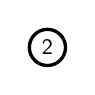
\begin{tikzpicture}[scale=.8, transform shape, level distance = 0.8cm]
    \tikzstyle{level 1}=[sibling distance=16mm]
    \tikzstyle{level 2}=[sibling distance=8mm]
    \node [avl_node] {2};
  \end{tikzpicture}
\end{minipage}
  \hspace{0.5cm}
  \begin{minipage}[c]{0.2\textwidth}
    \centering
    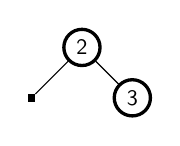
\begin{tikzpicture}[scale=.8, transform shape, level distance = 0.8cm]
      \tikzstyle{level 1}=[sibling distance=16mm]
      \tikzstyle{level 2}=[sibling distance=8mm]
      \node [avl_node] {2}
        child{ node [nil_leaf] {}}
        child{ node [avl_node] {3}};
    \end{tikzpicture}

      
  \end{minipage}
  \hspace{0.5cm}
  \begin{minipage}[c]{0.2\textwidth}
    \centering
    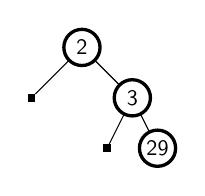
\begin{tikzpicture}[scale=.8, transform shape, level distance = 0.8cm]
      \tikzstyle{level 1}=[sibling distance=16mm]
      \tikzstyle{level 2}=[sibling distance=8mm]
      \node [avl_node] {2}
          child{ node [nil_leaf] {}}
          child{ node [avl_node] {3}
            child{ node [nil_leaf] {} }
            child{ node [avl_node] {29} }
          }
      ;
    \end{tikzpicture}
  \end{minipage}
  \hspace{0.5cm}
  \begin{minipage}[c]{0.2\textwidth}
    \centering
    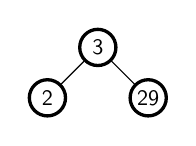
\begin{tikzpicture}[scale=.8, transform shape, level distance = 0.8cm]
      \tikzstyle{level 1}=[sibling distance=16mm]
      \tikzstyle{level 2}=[sibling distance=8mm]
      \node [avl_node] {3}
        child{ node [avl_node] {2}}
        child{ node [avl_node] {29}};
    \end{tikzpicture}
  \end{minipage}



\begin{minipage}[c]{0.2\textwidth}
  \centering
  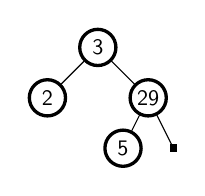
\begin{tikzpicture}[scale=.8, transform shape, level distance = 0.8cm]
    \tikzstyle{level 1}=[sibling distance=16mm]
    \tikzstyle{level 2}=[sibling distance=8mm]
    \node [avl_node] {3}
      child{ node [avl_node] {2} }
      child{ node [avl_node] {29}
        child{ node [avl_node] {5} }
        child{ node [nil_leaf] {} }
      }
    ;
  \end{tikzpicture}
\end{minipage}
  \hspace{0.5cm}
  \begin{minipage}[c]{0.2\textwidth}
    \centering
    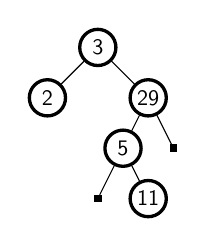
\begin{tikzpicture}[scale=.8, transform shape, level distance = 0.8cm]
      \tikzstyle{level 1}=[sibling distance=16mm]
      \tikzstyle{level 2}=[sibling distance=8mm]
      \node [avl_node] {3}
          child{ node [avl_node] {2}}
          child{ node [avl_node] {29}
            child{ node [avl_node] {5} 
                child{ node [nil_leaf] {}}
                child{ node [avl_node] {11} }
            }
            child{ node [nil_leaf] {}}
          }
      ;
    \end{tikzpicture}
  \end{minipage}
  \hspace{0.5cm}
  \begin{minipage}[c]{0.2\textwidth}
    \centering
    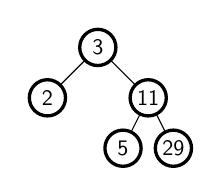
\begin{tikzpicture}[scale=.8, transform shape, level distance = 0.8cm]
      \tikzstyle{level 1}=[sibling distance=16mm]
      \tikzstyle{level 2}=[sibling distance=8mm]
      \node [avl_node] {3}
          child{ node [avl_node] {2}}
          child{ node [avl_node] {11}
            child{ node [avl_node] {5} }
            child{ node [avl_node] {29} }
          }
      ;
    \end{tikzpicture}
    
  \end{minipage}
  \hspace{0.5cm}
  \begin{minipage}[c]{0.2\textwidth}
    \centering
    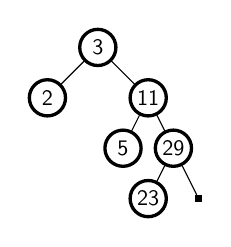
\begin{tikzpicture}[scale=.8, transform shape, level distance = 0.8cm]
      \tikzstyle{level 1}=[sibling distance=16mm]
      \tikzstyle{level 2}=[sibling distance=8mm]
      \node [avl_node] {3}
          child{ node [avl_node] {2}}
          child{ node [avl_node] {11}
            child{ node [avl_node] {5}}
            child{ node [avl_node] {29}
                child{ node [avl_node] {23}}
                child{ node [nil_leaf] {} }
            }
          }
      ;
    \end{tikzpicture}
  \end{minipage}




\begin{minipage}[c]{0.2\textwidth}
  \centering
  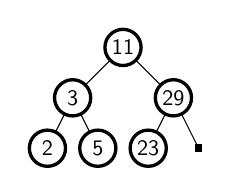
\begin{tikzpicture}[scale=.8, transform shape, level distance = 0.8cm]
    \tikzstyle{level 1}=[sibling distance=16mm]
    \tikzstyle{level 2}=[sibling distance=8mm]
    \node [avl_node] {11}
      child{ node [avl_node] {3}
        child{ node [avl_node] {2} }
        child{ node [avl_node] {5} }
      }
      child{ node [avl_node] {29}
        child{ node [avl_node] {23} }
        child{ node [nil_leaf] {} }
      }
    ;
  \end{tikzpicture}
\end{minipage}
  \hspace{0.5cm}
  \begin{minipage}[c]{0.2\textwidth}
    \centering
    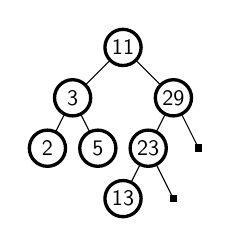
\begin{tikzpicture}[scale=.8, transform shape, level distance = 0.8cm]
      \tikzstyle{level 1}=[sibling distance=16mm]
      \tikzstyle{level 2}=[sibling distance=8mm]
      \node [avl_node] {11}
          child{ node [avl_node] {3}
            child{ node [avl_node] {2}}
            child{ node [avl_node] {5} }
          }
          child{ node [avl_node] {29}
            child{ node [avl_node] {23} 
                child{ node [avl_node] {13}}
                child{ node [nil_leaf] {} }
            }
            child{ node [nil_leaf] {} }
          }
      ;
    \end{tikzpicture}
  \end{minipage}
  \hspace{0.5cm}
  \begin{minipage}[c]{0.2\textwidth}
    \centering
    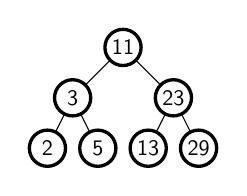
\begin{tikzpicture}[scale=.8, transform shape, level distance = 0.8cm]
      \tikzstyle{level 1}=[sibling distance=16mm]
      \tikzstyle{level 2}=[sibling distance=8mm]
      \node [avl_node] {11}
          child{ node [avl_node] {3}
            child{ node [avl_node] {2}}
            child{ node [avl_node] {5} }
          }
          child{ node [avl_node] {23}
            child{ node [avl_node] {13}}
            child{ node [avl_node] {29} }
          }
      ;
    \end{tikzpicture}
  \end{minipage}
  \hspace{0.5cm}
  \begin{minipage}[c]{0.2\textwidth}
    \centering
    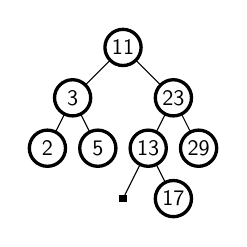
\begin{tikzpicture}[scale=.8, transform shape, level distance = 0.8cm]
      \tikzstyle{level 1}=[sibling distance=16mm]
      \tikzstyle{level 2}=[sibling distance=8mm]
      \node [avl_node] {11}
          child{ node [avl_node] {3}
            child{ node [avl_node] {2}}
            child{ node [avl_node] {5} }
          }
          child{ node [avl_node] {23}
            child{ node [avl_node] {13}
                child{ node [nil_leaf] {}}
                child{ node [avl_node] {17} }
            }
            child{ node [avl_node] {29} }
          }
      ;
    \end{tikzpicture}
  \end{minipage}



\begin{minipage}[c]{0.2\textwidth}
    \centering
    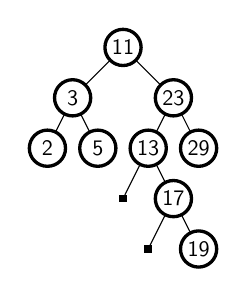
\begin{tikzpicture}[scale=.8, transform shape, level distance = 0.8cm]
      \tikzstyle{level 1}=[sibling distance=16mm]
      \tikzstyle{level 2}=[sibling distance=8mm]
      \node [avl_node] {11}
          child{ node [avl_node] {3}
            child{ node [avl_node] {2}}
            child{ node [avl_node] {5} }
          }
          child{ node [avl_node] {23}
            child{ node [avl_node] {13}
                child{ node [nil_leaf] {}}
                child{ node [avl_node] {17} 
                    child{ node [nil_leaf] {}}
                    child{ node [avl_node] {19} }
                }
            }
            child{ node [avl_node] {29} }
          }
      ;
    \end{tikzpicture}
  \end{minipage}
  \hspace{0.5cm}
  \begin{minipage}[c]{0.2\textwidth}
    \centering
    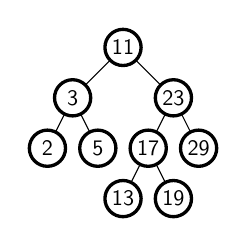
\begin{tikzpicture}[scale=.8, transform shape, level distance = 0.8cm]
      \tikzstyle{level 1}=[sibling distance=16mm]
      \tikzstyle{level 2}=[sibling distance=8mm]
      \node [avl_node] {11}
          child{ node [avl_node] {3}
            child{ node [avl_node] {2}}
            child{ node [avl_node] {5} }
          }
          child{ node [avl_node] {23}
            child{ node [avl_node] {17}
                child{ node [avl_node] {13}}
                child{ node [avl_node] {19}}
            }
            child{ node [avl_node] {29} }
          }
      ;
    \end{tikzpicture}
  \end{minipage}
\hspace{0.5cm}
\begin{minipage}[c]{0.3\textwidth}
  \centering
  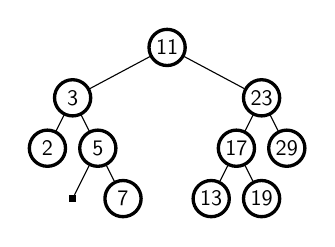
\begin{tikzpicture}[scale=.8, transform shape]
    \tikzstyle{level 1}=[sibling distance=30mm, level distance=0.8cm]
    \tikzstyle{level 2}=[sibling distance=8mm, level distance=0.8cm]

    \node [avl_node] {11}
      child{ node [avl_node] {3}
        child{ node [avl_node] {2} }
        child{ node [avl_node] {5}
          child{ node [nil_leaf] {} }
          child{ node [avl_node] {7} }
        }
      }
      child{ node [avl_node] {23}
        child{ node [avl_node] {17}
          child{ node [avl_node] {13} }
          child{ node [avl_node] {19} }
        }
        child{ node [avl_node] {29} }
      }
    ;
  \end{tikzpicture}
\end{minipage}


\begin{itemize}
\begin{minipage}[c]{0.5\textwidth}
      
      \textbf{The tables contains only balanced arrays:}
    \end{minipage}
  \item[\textbf{1)}] 
    \begin{minipage}[c]{0.01\textwidth}
      \centering
      \begin{tabular}{|c|c|c|c|c|c|c|}
        \hline
        \makebox[\widthof{0}][c]{2} \\
        \hline
      \end{tabular}
    \end{minipage}
    \hspace{3mm}
    \text{-- 0 rotation at this step}
  \item[\textbf{2)}] 
    \begin{minipage}[c]{0.1\textwidth}
      \centering
      \begin{tabular}{|c|c|c|c|c|c|c|c|c|c|c|c|c|c|c|}
        \hline
        \makebox[\widthof{0}][c]{2} &
        \makebox[\widthof{0}][c]{-} &
        \makebox[\widthof{0}][c]{3} \\
        \hline
      \end{tabular}
    \end{minipage}
    \hspace{1mm}
    \text{-- 0 rotation at this step}
    \item[\textbf{3)}] 
    \begin{minipage}[c]{0.1\textwidth}
      \centering
      \begin{tabular}{|c|c|c|c|c|c|c|}
        \hline
        \makebox[\widthof{0}][c]{3} &
        \makebox[\widthof{0}][c]{2} &
        \makebox[\widthof{0}][c]{29} \\
        \hline
      \end{tabular}
    \end{minipage}
    \hspace{1mm}
    \text{-- 1 rotation at this step}
    \item[\textbf{4)}] 
    \begin{minipage}[c]{0.1\textwidth}
      \centering
      \begin{tabular}{|c|c|c|c|c|c|c|}
        \hline
        \makebox[\widthof{0}][c]{3} &
        \makebox[\widthof{0}][c]{2} &
        \makebox[\widthof{0}][c]{29} &
        \makebox[\widthof{0}][c]{-} &
        \makebox[\widthof{0}][c]{-} &
        \makebox[\widthof{0}][c]{5} &
        \makebox[\widthof{0}][c]{-} \\
        \hline
      \end{tabular}
    \end{minipage}
    \hspace{25mm}
    \text{-- 0 rotation at this step}
    \item[\textbf{5)}] 
    \begin{minipage}[c]{0.1\textwidth}
      \centering
      \begin{tabular}{|c|c|c|c|c|c|c|}
        \hline
        \makebox[\widthof{0}][c]{3} &
        \makebox[\widthof{0}][c]{2} &
        \makebox[\widthof{0}][c]{11} &
        \makebox[\widthof{0}][c]{-} &
        \makebox[\widthof{0}][c]{-} &
        \makebox[\widthof{0}][c]{5} &
        \makebox[\widthof{0}][c]{29} \\
        \hline
      \end{tabular}
    \end{minipage}
    \hspace{25mm}
    \text{-- 2 rotation at this step}
    \item[\textbf{6)}] 
    \begin{minipage}[c]{0.1\textwidth}
      \centering
      \begin{tabular}{|c|c|c|c|c|c|c|}
        \hline
        \makebox[\widthof{0}][c]{11} &
        \makebox[\widthof{0}][c]{3} &
        \makebox[\widthof{0}][c]{29} &
        \makebox[\widthof{0}][c]{2} &
        \makebox[\widthof{0}][c]{5} &
        \makebox[\widthof{0}][c]{23} &
        \makebox[\widthof{0}][c]{-} \\
        \hline
      \end{tabular}
    \end{minipage}
    \hspace{25mm}
    \text{-- 1 rotation at this step}
    \item[\textbf{7)}] 
    \begin{minipage}[c]{0.1\textwidth}
      \centering
      \begin{tabular}{|c|c|c|c|c|c|c|}
        \hline
        \makebox[\widthof{0}][c]{11} &
        \makebox[\widthof{0}][c]{3} &
        \makebox[\widthof{0}][c]{23} &
        \makebox[\widthof{0}][c]{2} &
        \makebox[\widthof{0}][c]{5} &
        \makebox[\widthof{0}][c]{13} &
        \makebox[\widthof{0}][c]{29} \\
        \hline
      \end{tabular}
    \end{minipage}
    \hspace{25mm}
    \text{-- 1 rotation at this step}
    \item[\textbf{8)}] 
    \begin{minipage}[c]{0.1\textwidth}
      \centering
      \begin{tabular}{|c|c|c|c|c|c|c|c|c|c|c|c|c|c|c|c|c|c|c|c|c|}
        \hline
        \makebox[\widthof{0}][c]{11} &
        \makebox[\widthof{0}][c]{3} &
        \makebox[\widthof{0}][c]{23} &
        \makebox[\widthof{0}][c]{2} &
        \makebox[\widthof{0}][c]{5} &
        \makebox[\widthof{0}][c]{13} &
        \makebox[\widthof{0}][c]{29} &
        \makebox[\widthof{0}][c]{-} &
        \makebox[\widthof{0}][c]{-} &
        \makebox[\widthof{0}][c]{-} &
        \makebox[\widthof{0}][c]{-} &
        \makebox[\widthof{0}][c]{-} &
        \makebox[\widthof{0}][c]{17} &
        \makebox[\widthof{0}][c]{-}  &
        \makebox[\widthof{0}][c]{-} \\
        \hline
      \end{tabular}
    \end{minipage}
    \hspace{73mm}
    \text{-- 0 rotation at this step}
    \item[\textbf{9)}] 
    \begin{minipage}[c]{0.1\textwidth}
      \centering
      \begin{tabular}{|c|c|c|c|c|c|c|c|c|c|c|c|c|c|c|c|c|c|c|c|c|}
        \hline
        \makebox[\widthof{0}][c]{11} &
        \makebox[\widthof{0}][c]{3} &
        \makebox[\widthof{0}][c]{23} &
        \makebox[\widthof{0}][c]{2} &
        \makebox[\widthof{0}][c]{5} &
        \makebox[\widthof{0}][c]{17} &
        \makebox[\widthof{0}][c]{29} &
        \makebox[\widthof{0}][c]{-} &
        \makebox[\widthof{0}][c]{-} &
        \makebox[\widthof{0}][c]{-} &
        \makebox[\widthof{0}][c]{-} &
        \makebox[\widthof{0}][c]{13} &
        \makebox[\widthof{0}][c]{19} &
        \makebox[\widthof{0}][c]{-}  &
        \makebox[\widthof{0}][c]{-} \\
        \hline
      \end{tabular}
    \end{minipage}
    \hspace{73mm}
    \text{-- 1 rotation at this step}
    \item[\textbf{10)}] 
    \begin{minipage}[c]{0.1\textwidth}
      \centering
      \begin{tabular}{|c|c|c|c|c|c|c|c|c|c|c|c|c|c|c|c|c|c|c|c|c|}
        \hline
        \makebox[\widthof{0}][c]{11} &
        \makebox[\widthof{0}][c]{3} &
        \makebox[\widthof{0}][c]{23} &
        \makebox[\widthof{0}][c]{2} &
        \makebox[\widthof{0}][c]{5} &
        \makebox[\widthof{0}][c]{17} &
        \makebox[\widthof{0}][c]{29} &
        \makebox[\widthof{0}][c]{-} &
        \makebox[\widthof{0}][c]{-} &
        \makebox[\widthof{0}][c]{-} &
        \makebox[\widthof{0}][c]{7} &
        \makebox[\widthof{0}][c]{13} &
        \makebox[\widthof{0}][c]{19} &
        \makebox[\widthof{0}][c]{-}  &
        \makebox[\widthof{0}][c]{-} \\
        \hline
      \end{tabular}
    \end{minipage}
    \hspace{73mm}
    \text{-- 0 rotation at this step}\\
    \begin{minipage}[c]{0.5\textwidth}
    \textbf{The number of rotations is 6}
\end{minipage}
\end{itemize}


  
    \color{black}
  \item Perform the following operations starting with a reb-black tree~\cite[\S 13]{Cormen2022} presented below:

  \begin{center}
    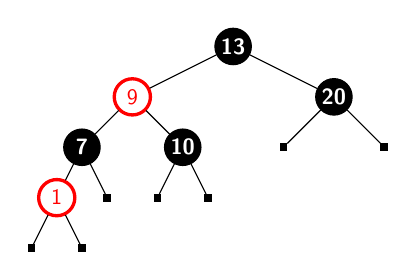
\begin{tikzpicture}[scale=.8, transform shape, level distance = 0.8cm]
      % [->,>=stealth',level/.style={sibling distance = 2cm/#1, level distance = 0.8cm}]
      \tikzstyle{level 1}=[sibling distance=32mm]
      \tikzstyle{level 2}=[sibling distance=16mm]
      \tikzstyle{level 3}=[sibling distance=8mm]
    \node [black_node] {13}
        child{ node [red_node] {9}
          child{ node [black_node] {7}
            child{ node [red_node] {1}
              child{ node [nil_leaf] {} }
              child{ node [nil_leaf] {} }
            }
            child{ node [nil_leaf] {} }
          }
          child{ node [black_node] {10}
            child{ node [nil_leaf] {} }
            child{ node [nil_leaf] {} }
          }
        }
        child{ node [black_node] {20}
          child{ node [nil_leaf] {} }
          child{ node [nil_leaf] {} }
        }
    ;
    \end{tikzpicture}
    \end{center}

    \begin{itemize}
      \item insert $18, 5, 7$
      \item insert $25, 20, 24$
      \item insert $23, 22, 21$
      \item delete $5, 9, 23$
      \item delete $22, 31, 1$
    \end{itemize}

    For each triple of operations (insertions or deletions):
    \begin{itemize}
      \item show the \emph{state of the tree} \textbf{after} the operations
      \item specify the total \emph{number of rotations} performed during the operations
    \end{itemize}

    Depict each tree using the array representation for binary trees.
    You \textbf{must} color the keys for red nodes with \textbf{\color{red}red} and keys for black nodes with \textbf{\color{black}black} color.
    For example, the initial red-black tree presented above is depicted as the following array:

    \begin{center}
    \begin{tabular}{|c|c|c|c|c|c|c|c|c|c|c|c|c|c|c|}
      \hline
        \makebox[\widthof{0}][c]{\textbf{\color{black}13}}
      & \makebox[\widthof{0}][c]{\textbf{\color{red}9}}
      & \makebox[\widthof{0}][c]{\textbf{\color{black}20}}
      & \makebox[\widthof{0}][c]{\textbf{\color{black}7}}
      & \makebox[\widthof{0}][c]{\textbf{\color{black}10}}
      & \makebox[\widthof{0}][c]{--}
      & \makebox[\widthof{0}][c]{--}
      & \makebox[\widthof{0}][c]{\textbf{\color{red}1}}
      & \makebox[\widthof{0}][c]{--}
      & \makebox[\widthof{0}][c]{--}
      & \makebox[\widthof{0}][c]{--}
      & \makebox[\widthof{0}][c]{--}
      & \makebox[\widthof{0}][c]{--}
      & \makebox[\widthof{0}][c]{--}
      & \makebox[\widthof{0}][c]{--}
      \\
      \hline
    \end{tabular}
    \end{center}

    \color{blue}
    \textbf{Answer:} \textbf{Total of 12 rotations}


\begin{itemize}

    \item[\textbf{1)}]
    \textbf{Total of 3 rotations and 3 rotations at step 1}\\
\begin{minipage}[c]{0.01\textwidth}
      \centering
      \begin{tabular}{|c|c|c|c|c|c|c|c|c|c|c|c|c|c|c|}
      \hline
        \makebox[\widthof{0}][c]{\textbf{\color{black}9}}
      & \makebox[\widthof{0}][c]{\textbf{\color{red}5}}
      & \makebox[\widthof{0}][c]{\textbf{\color{red}13}}
      & \makebox[\widthof{0}][c]{\textbf{\color{black}1}}
      & \makebox[\widthof{0}][c]{\textbf{\color{black}7}}
      & \makebox[\widthof{0}][c]{\textbf{\color{black}10}}
      & \makebox[\widthof{0}][c]{\textbf{\color{black}20}}
      & \makebox[\widthof{0}][c]{--}
      & \makebox[\widthof{0}][c]{--}
      & \makebox[\widthof{0}][c]{--}
      & \makebox[\widthof{0}][c]{\textbf{\color{red}7}}
      & \makebox[\widthof{0}][c]{--}
      & \makebox[\widthof{0}][c]{--}
      & \makebox[\widthof{0}][c]{\textbf{\color{red}18}}
      & \makebox[\widthof{0}][c]{--}
      \\
      \hline
    \end{tabular}
    \end{minipage}
    
\end{itemize}
\begin{itemize}
    \item[\textbf{2)}]
    \textbf{Total of 5 rotations and 2 rotations at step 2}\\ 
    \begin{tabular}{|c|c|c|c|c|c|c|c|c|c|c|c|c|c|c}
      \hline
        \makebox[\widthof{0}][c]{\textbf{\color{black}9}}
      & \makebox[\widthof{0}][c]{\textbf{\color{black}5}}
      & \makebox[\widthof{0}][c]{\textbf{\color{black}13}}
      & \makebox[\widthof{0}][c]{\textbf{\color{black}1}}
      & \makebox[\widthof{0}][c]{\textbf{\color{black}7}}
      & \makebox[\widthof{0}][c]{\textbf{\color{black}10}}
      & \makebox[\widthof{0}][c]{\textbf{\color{red}20}}
      & \makebox[\widthof{0}][c]{--}
      & \makebox[\widthof{0}][c]{--}
      & \makebox[\widthof{0}][c]{--}
      & \makebox[\widthof{0}][c]{\textbf{\color{red}7}}
      & \makebox[\widthof{0}][c]{--}
      & \makebox[\widthof{0}][c]{--}
      & \makebox[\widthof{0}][c]{\textbf{\color{black}18}}
      & \makebox[\widthof{0}][c]{\textbf{\color{black}24}}
      \\
      \hline
    \end{tabular}
    \Rightarrow\\
    \begin{flushright}
        \begin{tabular}{|c|c|c|c|c|c|c|c|c|c|c|c|c|c|c|c|c|c|c|c|c|c|c|c|}
          \hline
           \makebox[\widthof{0}][c]{--}
          & \makebox[\widthof{0}][c]{--}
          & \makebox[\widthof{0}][c]{--}
          & \makebox[\widthof{0}][c]{--}
          
          & \makebox[\widthof{0}][c]{--}
          & \makebox[\widthof{0}][c]{--}
          & \makebox[\widthof{0}][c]{--}
          & \makebox[\widthof{0}][c]{--}
          
          & \makebox[\widthof{0}][c]{--}
          & \makebox[\widthof{0}][c]{--}
          & \makebox[\widthof{0}][c]{--}
          & \makebox[\widthof{0}][c]{--}
            & \makebox[\widthof{0}][c]{--}
          & \makebox[\widthof{0}][c]{--}
          &\makebox[\widthof{0}][c]{\textbf{\color{red}20}}
          & \makebox[\widthof{0}][c]{\textbf{\color{red}25}}
          \\
          \hline
        \end{tabular}
    \end{flushright}
\end{itemize}
\begin{itemize}
    \item[\textbf{3)}]
    \textbf{Total of 8 rotations and 3 rotations at step 3}\\   
        \begin{tabular}{|c|c|c|c|c|c|c|c|c|c|c|c|c|c|c}
          \hline
            \makebox[\widthof{0}][c]{\textbf{\color{black}9}}
          & \makebox[\widthof{0}][c]{\textbf{\color{black}5}}
          & \makebox[\widthof{0}][c]{\textbf{\color{red}20}}
          & \makebox[\widthof{0}][c]{\textbf{\color{black}1}}
          & \makebox[\widthof{0}][c]{\textbf{\color{black}7}}
          & \makebox[\widthof{0}][c]{\textbf{\color{black}13}}
          & \makebox[\widthof{0}][c]{\textbf{\color{black}24}}
          & \makebox[\widthof{0}][c]{--}
          & \makebox[\widthof{0}][c]{--}
          & \makebox[\widthof{0}][c]{--}
          & \makebox[\widthof{0}][c]{\textbf{\color{red}7}}
          & \makebox[\widthof{0}][c]{\textbf{\color{black}10}}
          & \makebox[\widthof{0}][c]{\textbf{\color{black}18}}
          & \makebox[\widthof{0}][c]{\textbf{\color{red}22}}
          & \makebox[\widthof{0}][c]{\textbf{\color{black}25}}
          \\
          \hline
        \end{tabular}
    \Rightarrow\\
    \begin{flushright}
        \begin{tabular}{|c|c|c|c|c|c|c|c|c|c|c|c|c|c|c|c}
          \hline
           \makebox[\widthof{0}][c]{--}
          & \makebox[\widthof{0}][c]{--}
          & \makebox[\widthof{0}][c]{--}
          & \makebox[\widthof{0}][c]{--}
          & \makebox[\widthof{0}][c]{--}
          & \makebox[\widthof{0}][c]{--}
          & \makebox[\widthof{0}][c]{--}
          & \makebox[\widthof{0}][c]{--}
          & \makebox[\widthof{0}][c]{--}
          & \makebox[\widthof{0}][c]{--}
          & \makebox[\widthof{0}][c]{--}
           & \makebox[\widthof{0}][c]{--}
          & \makebox[\widthof{0}][c]{\textbf{\color{black}20}}
          & \makebox[\widthof{0}][c]{\textbf{\color{black}23}}
          & \makebox[\widthof{0}][c]{--}
          & \makebox[\widthof{0}][c]{--}
          \\
          \hline
        \end{tabular}
    \Rightarrow\\
        \begin{tabular}{|c|c|c|c|c|c|c|c|c|c|c|c|c|c|c|c}
          \hline
           \makebox[\widthof{0}][c]{--}
          & \makebox[\widthof{0}][c]{--}
          & \makebox[\widthof{0}][c]{--}
          & \makebox[\widthof{0}][c]{--}
          
          & \makebox[\widthof{0}][c]{--}
          & \makebox[\widthof{0}][c]{--}
          & \makebox[\widthof{0}][c]{--}
          & \makebox[\widthof{0}][c]{--}
          
          & \makebox[\widthof{0}][c]{--}
          & \makebox[\widthof{0}][c]{--}
          & \makebox[\widthof{0}][c]{--}
           & \makebox[\widthof{0}][c]{--}
           
          & \makebox[\widthof{0}][c]{--}
           & \makebox[\widthof{0}][c]{--}
          & \makebox[\widthof{0}][c]{--}
          & \makebox[\widthof{0}][c]{--}
          \\
          \hline
        \end{tabular}
        \Rightarrow\\
        \begin{tabular}{|c|c|c|c|c|c|c|c|c|c|c|c|c|c|c|c|c|c|c|}
          \hline
           \makebox[\widthof{0}][c]{--}
          & \makebox[\widthof{0}][c]{--}
          & \makebox[\widthof{0}][c]{--}
          & \makebox[\widthof{0}][c]{--}
          
          & \makebox[\widthof{0}][c]{--}
          & \makebox[\widthof{0}][c]{--}
          & \makebox[\widthof{0}][c]{--}
          & \makebox[\widthof{0}][c]{--}
          
          & \makebox[\widthof{0}][c]{--}
          & \makebox[\widthof{0}][c]{\textbf{\color{red}21}}
          & \makebox[\widthof{0}][c]{--}
           & \makebox[\widthof{0}][c]{--}
           
          & \makebox[\widthof{0}][c]{--}
           & \makebox[\widthof{0}][c]{--}
          & \makebox[\widthof{0}][c]{--}
          & \makebox[\widthof{0}][c]{--}
          \\
          \hline
        \end{tabular}
    \end{flushright}
\end{itemize}
\begin{itemize}
    \item[\textbf{4)}]
    \textbf{Total of 12 rotations and 4 rotations at step 4}\\  
        \begin{tabular}{|c|c|c|c|c|c|c|c|c|c|c|c|c|c|c|}
          \hline
            \makebox[\widthof{0}][c]{\textbf{\color{black}20}}
          & \makebox[\widthof{0}][c]{\textbf{\color{black}7}}
          & \makebox[\widthof{0}][c]{\textbf{\color{black}24}}
          & \makebox[\widthof{0}][c]{\textbf{\color{black}7}}
          & \makebox[\widthof{0}][c]{\textbf{\color{red}13}}
          & \makebox[\widthof{0}][c]{\textbf{\color{red}21}}
          & \makebox[\widthof{0}][c]{\textbf{\color{black}25}}
          & \makebox[\widthof{0}][c]{\textbf{\color{red}1}}
          & \makebox[\widthof{0}][c]{--}
          & \makebox[\widthof{0}][c]{\textbf{\color{black}10}}
          & \makebox[\widthof{0}][c]{\textbf{\color{black}18}}
          & \makebox[\widthof{0}][c]{\textbf{\color{black}20}}
          & \makebox[\widthof{0}][c]{\textbf{\color{black}22}}
          & \makebox[\widthof{0}][c]{--}
          & \makebox[\widthof{0}][c]{--}
          \\
          \hline
        \end{tabular}
\end{itemize}
\begin{itemize}
    \item[\textbf{5)}]
    \textbf{Total of 12 rotations and 0 rotations at step 5}\\ 
        \begin{tabular}{|c|c|c|c|c|c|c|c|c|c|c|c|c|c|c|}
          \hline
            \makebox[\widthof{0}][c]{\textbf{\color{black}20}}
          & \makebox[\widthof{0}][c]{\textbf{\color{black}7}}
          & \makebox[\widthof{0}][c]{\textbf{\color{black}24}}
          & \makebox[\widthof{0}][c]{\textbf{\color{black}7}}
          & \makebox[\widthof{0}][c]{\textbf{\color{red}13}}
          & \makebox[\widthof{0}][c]{\textbf{\color{black}21}}
          & \makebox[\widthof{0}][c]{\textbf{\color{black}25}}
          & \makebox[\widthof{0}][c]{--}
          & \makebox[\widthof{0}][c]{--}
          & \makebox[\widthof{0}][c]{\textbf{\color{black}10}}
          & \makebox[\widthof{0}][c]{\textbf{\color{black}18}}
          & \makebox[\widthof{0}][c]{\textbf{\color{red}20}}
          & \makebox[\widthof{0}][c]{--}
          & \makebox[\widthof{0}][c]{--}
          & \makebox[\widthof{0}][c]{--}
          \\
          \hline
        \end{tabular}
\end{itemize}

    
    \color{black}

  \clearpage
  \item Compare randomly-built binary search trees and randomly chosen binary search trees for size $n = 4$:
  \begin{enumerate}
    \item Write down the number of distinct shapes for a binary search trees of size $n = 4$.
      \color{blue}\\
      \textbf{Answer:} 14




      
      \color{black}
    \item What is the average height of a randomly chosen binary search tree of size $n = 4$?
    \color{blue}\\
    \textbf{Answer:} $\frac{18}{7} = 2 \frac{4}{7} \approx 3$
    \color{black}
    \item Consider $a < b < c < d$. For every permutation of $a, b, c, d$, write down an array representation of a corresponding
    binary search tree built from that permutation (by inserting keys in the given order).
    \color{blue}
      \textbf{Answer:}


        \begin{tabular}{|c||c|c||c|c|c|c||c|c|c|c|c|c|c|c|}
    \hline
    \textbf{1} & \textbf{2} & \textbf{3} & \textbf{4} & \textbf{5} & \textbf{6} & \textbf{7} & \textbf{8} & \textbf{9} & \textbf{10} & \textbf{11} & \textbf{12} & \textbf{13} & \textbf{14} & \textbf{15} \\
    \hline
    \hline
    a & - & b & - & - & - & c & - & - & - & - & - & - & - & d \\
    \hline
    a & - & b & - & - & - & d & - & - & - & - & - & - & c & - \\
    \hline
    a & - & c & - & - & b & d  \\
    \cline{1-7}
    a & - & c & - & - & b & d  \\
    \hline
    a & - & d & - & - & b & - & - & - & - & - & - & c & - & - \\
    \hline
    a & - & d & - & - & c & - & - & - & - & - & b & - & - & - \\
    
    \hline
    
    b & a & c & - & - & - & d \\
    \cline{1-7}
    b & a & d & - & - & c & - \\
    \cline{1-7}
    b & a & c & - & - & - & d \\
    \cline{1-7}
    b & a & c & - & - & - & d \\
    \cline{1-7}
    b & a & d & - & - & c & - \\
    \cline{1-7}
    b & a & d & - & - & c & - \\
    
    \cline{1-7}
    
    c & a & d & - & b & - & - \\
    \cline{1-7}
    c & a & d & - & b & - & - \\
    \cline{1-7}
    c & b & d & a & - & - & - \\
    \cline{1-7}
    c & b & d & a & - & - & - \\
    \cline{1-7}
    c & a & d & - & b & - & - \\
    \cline{1-7}
    c & b & d & a & - & - & - \\

    
    \hline
    d & a & - & - & b & - & - & - & - & - & c & - & - & - & - \\
    \hline
    d & a & - & - & c & - & - & - & - & b & - & - & - & - & - \\
    \hline
    d & b & - & a & c & - & - \\
    \cline{1-7}
    d & b & - & a & c & - & - \\
    \hline
    d & c & - & a & - & - & - & - & b & - & - & - & - & - & - \\
    \hline
    d & c & - & b & - & - & - & a & - & - & - & - & - & - & - \\
    \hline
\end{tabular}



      
      \color{black}
    \item What is the average height of a randomly built binary search tree of size $n = 4$?
    \color{blue}\\
      \textbf{Answer:} $\frac{56}{24} = 2 \frac{1}{3} \approx 2$
      \color{black}
    \item Explain, in your own words, why we should not
      start with a complete binary tree of size $n$ (for any $n$)
      with ``empty'' nodes (i.e. each node does not have any key)
      and then populate it with given keys $k_1, k_2, \ldots, k_n$
      to achieve the optimal height of the resulting binary search tree.
      \color{blue}
      \textbf{Explanation:}\\
      Starting with a complete binary tree of size n and filling it with keys is a bad idea. If the keys are added in the wrong order (e.g., sorted), the tree becomes unbalanced (like a list), making search slow. This method ignores key order, so it’s not suitable for an efficient BST.
      \color{black}
  \end{enumerate}

\end{enumerate}

\begin{thebibliography}{BoasWrench}

\bibitem[CLRS]{Cormen2022}
Cormen, T.H., Leiserson, C.E., Rivest, R.L. and Stein, C., 2022. \emph{Introduction to algorithms, Fourth Edition}. MIT press.

\bibitem[GTG]{Goodrich2014}
M. T. Goodrich, R. Tamassia, and M. H. Goldwasser. \emph{Data Structures and Algorithms in Java.} WILEY 2014.

\end{thebibliography}

\end{document}